\chapter{Self-Organizing Algorithms for Resource Control in Autonomic Systems} % Write in your own chapter title
\label{Chapter_selforg}
\lhead{Chapter \ref{Chapter_selforg}. \emph{Self-Organizing Algorithms for Resource Control in Autonomic Systems}} % Write in your own chapter title to set the page header

The first step in the development of the self-organizing autonomic system is the development of the algorithms which will be used in order to control the resources (servers) in the autonomic system. This chapter will present two algorithms - one for predicting an SLA breach, and one for optimizing the size of the cloud once a breach is predicted.

\section{Self-organizing autonomic system for auto-scaling of cloud resources}

Due to the wide variety in applications which are deployed and run on clouds, a generic self-organizing system for cloud resources must be able to accept different measured inputs from the managed cloud application and perform the management of the cloud properly such that SLA breaches are minimized. Load for a server can be represented by a simple metric like CPU usage or memory usage or a complex combination of the number of clients connected to the server, the number of sessions running on the server, and the number of video streams received by the server and multiplexed towards receiving clients in the case of complex applications like the one presented in \cite{bogdan:miles2012chapter}. Based on the application's perturbations as noticed through the server load, each server can decide if it should receive more clients or not, independent of any decision made by another server. On top of this mechanism for server self-organization with relation to accepting new clients, the system also needs an approach to determine when the cluster's SLA will be breached and take proactive action by adding or removing servers from the cluster.

The reason to use a self-organizing systems for the adaptation of cloud resources is due to the intrinsic properties that self-organizing systems poses:
\begin{enumerate}
	\item Adaptable - the ability to deal with changes in the environment which were not predicted at design time. This is important for the system developed for the thesis as we do not know the bounds of how many servers could be in a cloud at one time or the maximum peak demand for the service and as such we want a system which is able to adapt the control law dynamically.
	\item Resilient - parts of the system can die or be lost but the remaining still perform their goal. In a cloud environment this is desired, as servers can come up an down at any time, and even network connectivity could be lost between servers or between data centers.
	\item Emergent - the complex behaviour arises from the properties and behaviour of the simple parts. As a cloud of servers increases in size it becomes more complicated for a single controller to manage the entire system. As such a system where the control emerges from the interactions of a lot of small parts is desired as it decreases complexity and can scale much more, at the cost of overall resource utilization.
	\item Anticipation - the system can anticipate problems and solve them before they impact the whole system. This is obviously desired, as we wish to detect SLA breaches before they happen, such that corrective actions can be taken and the breach can be avoided.
\end{enumerate}

From all of these the following requirements can be drawn for the system:

\begin{enumerate}
	\item The self-organizing system must be able to cope with different measurements which represent the load on one of the cloud's servers.
	\item The self-optimization is achieved without a central controller and only by the relation/communication between the self-organizing agents.
	\item The self-organizing system detects SLA breaches proactively such that it has time to react before the SLA is breached.
\end{enumerate}

The following sections will introduce the self-organizing system and the two self-organizing algorithms previously mentioned.

\section{Server self-optimization}

The first level of self-optimization for the system under control is each server's self-optimization. For the purpose of this thesis, the server self-optimization is quite simple: each server decides when to accept clients and when not to accept clients based on it's local knowledge and local control system. The control system used for each server is a fuzzy system which predicts the load on the server and based on the predicted load either stops accepting clients or starts accepting clients again if it had stopped before. For this purpose, each server has its own control loop, similar to the one developed in \cite{bogdan:seams07}. The architecture can be seen in Figure \ref{fig:selfopt-archi}. More complex control systems based on control theory can be used, however the control system for one server is not the main purpose of this thesis.

\begin{figure}
	\centering
	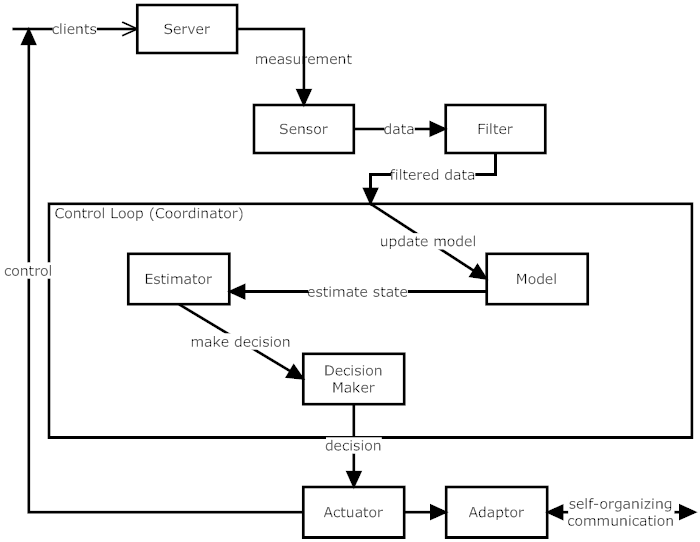
\includegraphics[width=0.9\linewidth]{Self-optimizingControlLoop_full}
	\caption{Self-Optimizing Control Loop Architecture}
	\label{fig:selfopt-archi}
\end{figure}

The fuzzy system will output a single metric representing the load of the server. This metric is then used by the self-organizing agents in order to predict an SLA breach and take actions to avoid the breach.

\section{SLA breach prediction: Ant Colony Optimization}

The ant colony optimization (ACO) algorithm \cite{antalgorithm}, \cite{selforg:aco} is best known for load balancing clouds or finding the best route in a network. The algorithm has received a lot of attention and work in academia and was presented in chapter \ref{Chapter_related}. At a high level the algorithm uses a number of simple agents called ants which traverse the network and leave a trail of pheromones which other ants can then follow. Good paths or solutions are reinforced by having more ants traverse them and leaving more pheromones. Once a path or solution is no longer viable, less ants travel it and another path is reinforced as more ants travel that path. In networking optimization ants behave as normal packets and traverse the network from router to router. When an ant reaches a router it can look at how long the arrival router's buffer queue is for the router the ant came from and then reinforce that route based on latency, buffer sizes, etc.

Take as an example a network that looks like the one in Figure \ref{fig:aco_init} in its initial non-traversed state, where the load of the links is the value shown on the edges of the graph, and in which ants start at node \textit{S} and finish at node \textit{E}. If there are 6 ants in the system, each ant deposits pheromone at a rate of $\frac{1}{edgeLoad}$, and in the initial state ants have an equal chance of taking an edge as there are no pheromones deposited, then the initial probability of an ant taking any given edge is shown in figure \ref{fig:aco_initprob}. Each edge in figure \ref{fig:aco_initprob} has a probability of being traversed by an ant of $\frac{1}{numberEdgesFromNode}$.

After the first run of the ants the pheromone in the network will look as in figure \ref{fig:aco_pher}. In figure \ref{fig:aco_pher} the edges show the number of ants taking each edge and the total amount of pheromone deposited in the form of $\frac{numberAnts}{totalPheomoneLevel}$. For example, the edge from \textit{S} to \textit{1} has 2 ants traversing it and total pheromone being deposited with a value of 2, while the edge from \textit{5} to \textit{6} has 2 ants traversing it and total pheromone being deposited with a value of 4 because the link has less load. While this example assumes that the ants split exactly as the probabilities shown in figure \ref{fig:aco_initprob}, note that it possible for more ants to take an edge with lower probability since ants roll a random value when deciding the edge to take.

When going back to the source, more ants will prefer edges with higher pheromone values thus resulting in that path being reinforced as shown in figure \ref{fig:aco_finalprob} where the probability of ants taking an edge is shown. This example does not include the decay of the pheromone level, but in an ACO implementation the pheromone level always decays at a given rate such that edges that are no longer traveled have their pheromone levels slowly decrease. As more time passes, ants will continue to add more pheromone on good paths in the end resulting in the path with the lowest load being reinforced. If the load in the network changes, ants will be able to start reinforcing the path with the better performance and forget about the previous path.

\begin{figure}
	\centering
	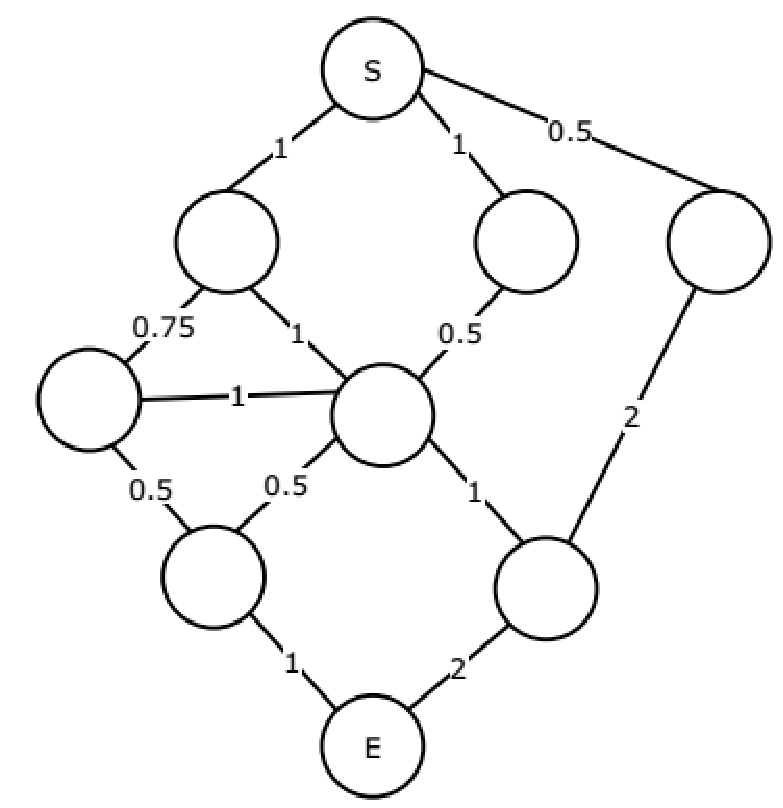
\includegraphics[width=0.9\linewidth]{aco_init}
	\caption{Network Ant Colony Optimization - Initial state}
	\label{fig:aco_init}
\end{figure}

\begin{figure}
	\centering
	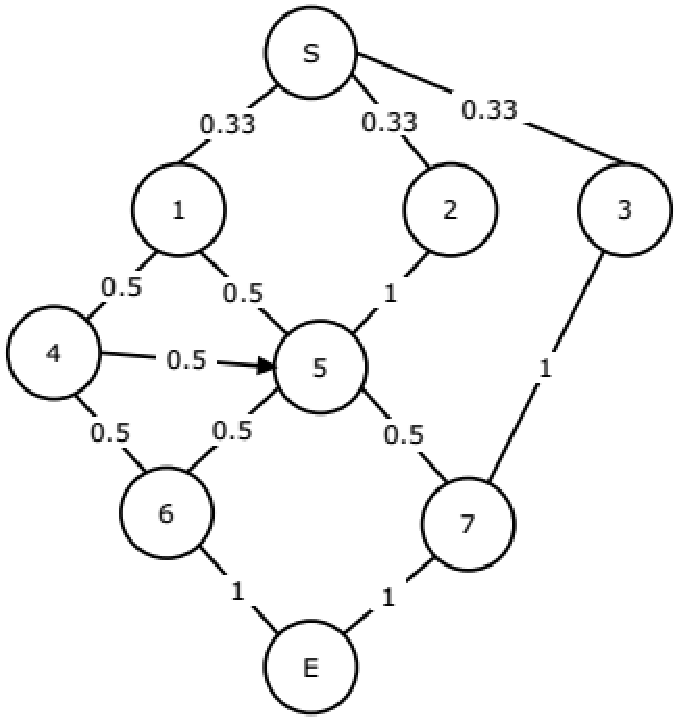
\includegraphics[width=0.9\linewidth]{aco_initprob}
	\caption{Network Ant Colony Optimization - Path probability initial}
	\label{fig:aco_initprob}
\end{figure}

\begin{figure}
	\centering
	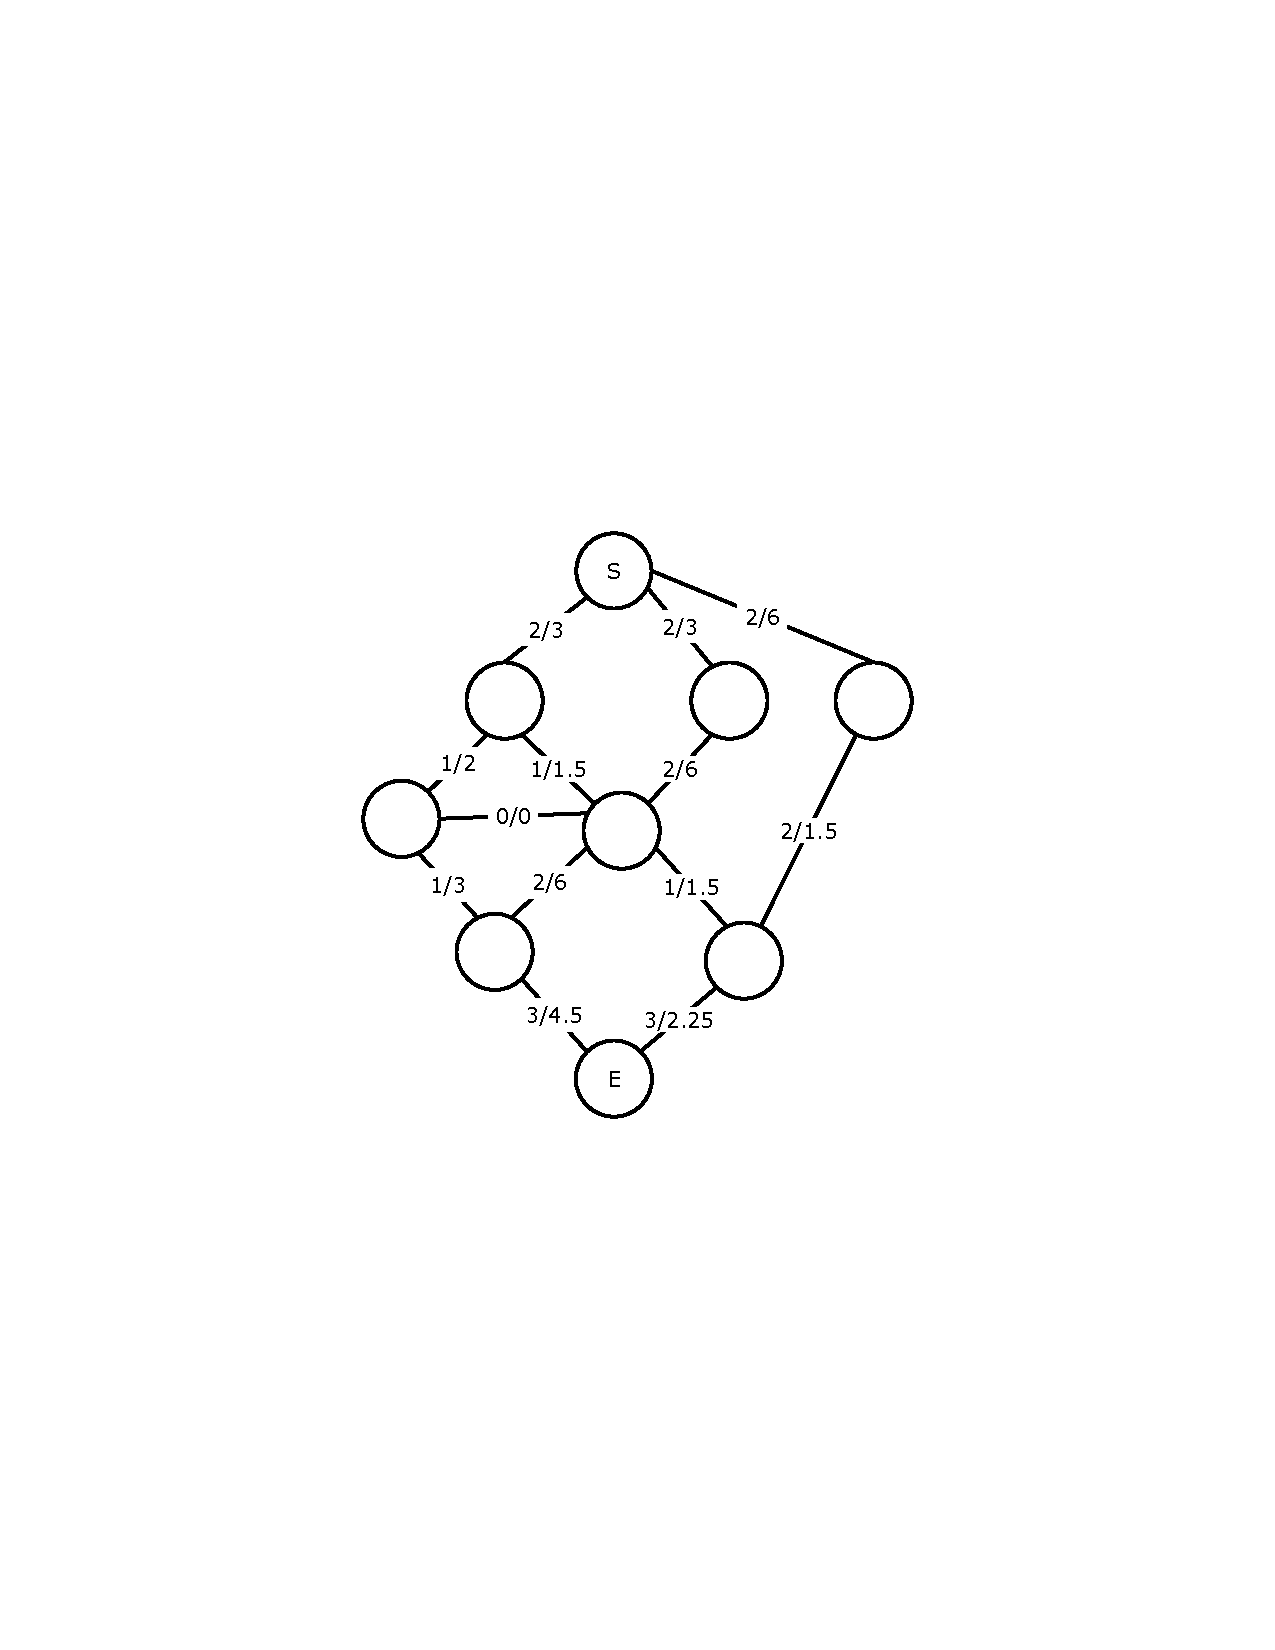
\includegraphics[width=0.9\linewidth]{aco_pher}
	\caption{Network Ant Colony Optimization - Pheromone update}
	\label{fig:aco_pher}
\end{figure}

\begin{figure}
	\centering
	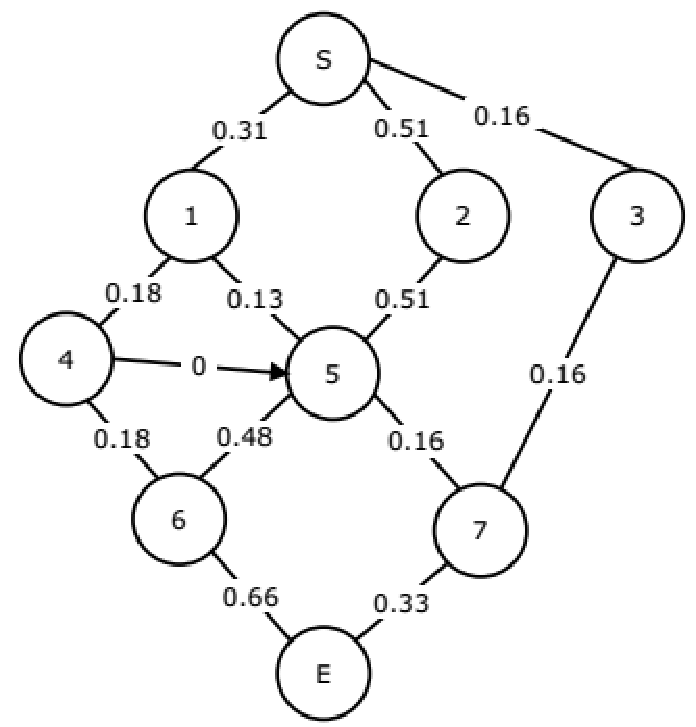
\includegraphics[width=0.9\linewidth]{aco_finalprob}
	\caption{Network Ant Colony Optimization - Path probability update}
	\label{fig:aco_finalprob}
\end{figure}

\subsection{ACO Model for SLA breach prediction}

The self-organizing algorithm used to predict SLA breaches in cloud systems is similar in nature to how the ACO algorithm behaves when finding the best route in a network. However, there are a number of significant differences due to the nature of the problem that is being resolved. The goal of the ACO algorithm while performing path optimization is to discover how viable different routes are and reinforce the good routes while at the same time diminishing the use of bad routes. For this problem the ants deposit pheromones on the routes between nodes such that paths with higher pheromones are more desired. In the case of the SLA breach prediction problem, the goal of the ACO algorithm is to determine based on the knowledge about the visited servers if the whole cloud is about to breach it's SLA requirements. For this problem, the ants deposit pheromones at the servers and use the amount of pheromone as a proxy of how loaded the whole cloud.

The ACO model for SLA breach prediction is composed of three components:

\begin{enumerate}
	\item Ants - ants are simple agents which traverse the network of servers and deposit pheromone at the servers based on a mathematical model
	\item Pheromone levels - each server has it's own pheromone level which is increased by ants visiting the server and decays periodically. Pheromones are a proxy of how overloaded a single server is.
	\item Mathematical model - this is the model which converts the fuzzy model result of each server into a pheromone value. The mathematical model also represents when an SLA breach is predicted.
\end{enumerate}

\subsection{Self-organizing agent: The ant}

Ants are simple agents that traverse the network of servers. They have no knowledge about the global state of the cloud and how overloaded all the servers in the cloud are. Ants only know the state at the currently visited server and also have a short memory about the last $x$ servers which the ant has visited and what the pheromone level was at those servers.

Whenever a server starts, the server's control system creates a new ant and sends it through the network of servers. Thus the total number of ants is equal to $N$ where $N$ is the number of live servers in the cloud. When an ant is first created, because it has no prior knowledge, it is sent to another server randomly. If only one server exists in the cloud, then the ant keeps visiting the same server.

As ants reach other servers they deposit pheromone at the server they arrive at, at a rate inversely proportional to the load of the server as represented by the fuzzy control system. At the same time ants wait at the server a time proportional to the load of the server. Thus overloaded servers will have less pheromone deposited when compared to an under-loaded server. By having ants wait a longer time at overloaded servers, the overall amount of pheromone in the network will further decrease. With this approach, a lower average amount of pheromone in the network of servers means that the cloud has higher load due to the fact that a larger number of servers have low pheromone levels because of being overloaded.

Ants also store information about the last $x$ servers the ant has visited and the time passed since the last visit to each of these servers. When an ant decides which server to go to, it uses a random function which is proportional to the time since it has visited a server combined with the pheromone level of the destination server. Thus the ant will give preference to the servers it has not visited in a long time, and especially the servers it has never visited or which are not in it's memory. Because the server structure is not stable and servers can join and leave at any time, ants decide the next server to visit based on the servers known by the current server the ant is at.  Assume a cloud with 5 servers and an ant which has the information in table \ref{tab:ant_prio} in it's history table and which reaches Server 5.

\begin{table}
\centering
\begin{tabular}{c|c|c}
Server & Time since last visit (s) & Pheromone Level \\
Server 1 & 15 & 10 \\ 
Server 2 & 20 & 5 \\
Server 3 & 5 & 8 \\
Server 4 & 35 & 5.5 \\
Server 5 & 0 & 10 \\
\end{tabular}
\caption{Ant routing knowledge prior}
\label{tab:ant_prio}
\end{table}

Based on the table, the ant computes the probability of visiting each server as:

\begin{equation}
P_s = (t_s / \sum_{i=1}^{N} t_i + p_{s} / \sum_{i=1}^{N} p_i) / 2
\end{equation}

where

\begin{equation}
i \in \left\{\text{servers known by current server the ant is at} \right\}
\end{equation}

where $P_s$ is the probability of visiting server $s$, $t_s$ is the time since it has visited server $s$ last time and $p_{s}$ is the pheromone at server $s$. These probabilities are computed only on the servers known as being up by the server the ant is at. The server the ant is currently at has to be excluded from the calculations, and it's visit probability will be 0. Assuming also that Server 5, which is the server the ant is at currently does not yet know about server 3. As such, the visit probability table looks as in Table \ref{tab:ant_prob}.

\begin{table}
\centering
\begin{tabular}{c|c}
Server & Probability (\%) \\
Server 1 & 35.10 \\
Server 2 & 26.48 \\
Server 4 & 38.42 \\
Server 5 & 0 \\
\end{tabular}
\caption{Ant routing probability}
\label{tab:ant_prob}
\end{table}

As such, the ant will roll a random value between 0 and 1, and choose which server to go to. A value between 0 and 0.3842 means that the next server will be \textit{Server 4}, between 0.3842 and 0.7352 it means that the next server will be \textit{Server 1} and a value between 0.7352 and 1 means \textit{Server 2}. Assuming the random value the ant rolls is 0.7, and that the ant waits at Server 5 for 5s and deposits 1 pheromone, the routing table after the ant moves to the next server will be as the one in Table \ref{tab:ant_post}.

\begin{table}
\centering
\begin{tabular}{c|c|c}
Server & Time since last visit (s) & Pheromone Level \\
Server 1 & 0 & 10 \\
Server 2 & 25 & 5 \\
Server 3 & 10 & 8 \\
Server 4 & 40 & 5.5 \\
Server 5 & 5 & 11 \\
\end{tabular}
\caption{Ant routing knowledge posterior}
\label{tab:ant_post}
\end{table}

In order to avoid having all ants visit a new node at the same time, whenever an ant discovers a new server it initializes the time since it visited the server with a random value. Assume that after the ant reaches Server 1, it discovers a new server which was unknown before - Server 6. The time since last visiting Server 6 will be initialized with a random value between 0 and the maximum time since last visiting a server which is known to be alive as in Equation \ref{eq:randomnew}. Furthermore the known pheromone level of the new server will be 0. If Server 1 only knows Server 2, 3 and 5 then the random value will be between 0 and 25s.

\begin{equation}
t_{new} = random(0, max(t_{known}))
\label{eq:randomnew}
\end{equation}

An ant's behaviour can be described by the algorithm below:

\begin{algorithm}
\begin{algorithmic}
	\State Calculate pheromone at current node
	\State Update ant's server history tables
	\If{Ant should morph}
		\State Morph ant
	\Else
		\State Calculate next server for ant
		\State Send ant to next server
	\EndIf
\end{algorithmic}
\caption{Ant Colony Optimization Pseudocode}\label{ant:pseudocode}
\end{algorithm}

For example, for a network of five servers Figure \ref{fig:antnetwork} shows the behaviour of the ant algorithm.

\begin{figure}
	\centering
	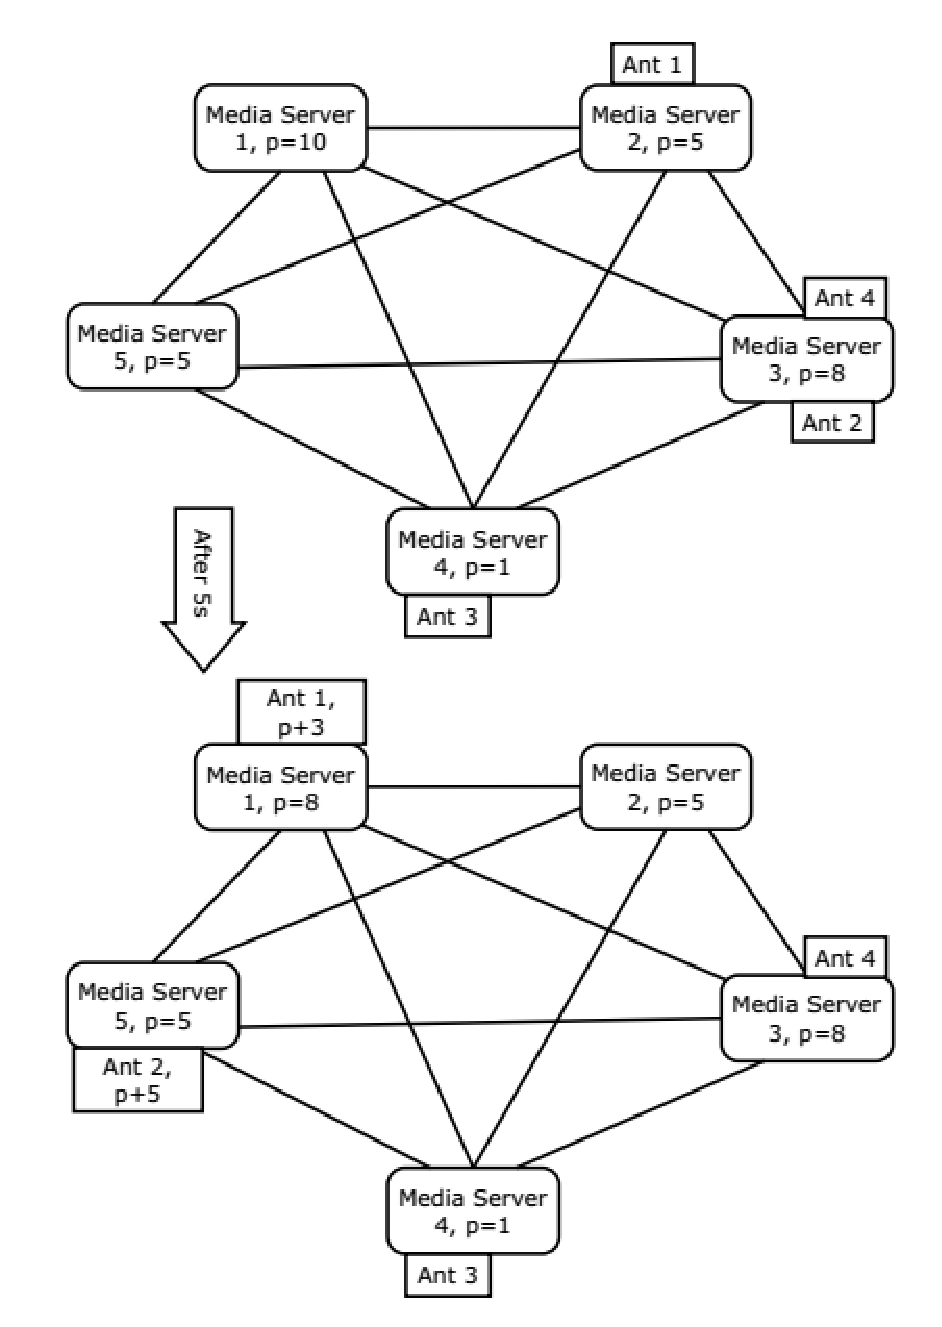
\includegraphics[width=0.9\linewidth]{aco_cloud}
	\caption{Ant Colony Optimization Network}
	\label{fig:antnetwork}
\end{figure}

\subsection{Server and cloud load: Pheromone levels}

For the purpose of controlling the number of servers in the cloud, the pheromone level in the network is used as a proxy for how loaded the entire cloud of servers is and is used to decide when to add or remove servers. As ants move through the network of servers they deposit pheromones - whenever an ant reaches a server it computes how much pheromone to deposit based on the result of the control system for that server. If the server's control system has a result which shows that the server is underloaded then more pheromone is deposited. If the server is overloaded then less pheromone is deposited. At the same time the pheromone amount at each server decays periodically at a constant rate. As such, a large amount of pheromone shows that servers are underloaded and servers should be removed, while a small amount of pheromone shows that servers are overloaded and that servers should be added.

On top of updating the pheromone at each server, each ant is also responsible for measuring the pheromone level at each node it visits. Ants store a history of the last $x$ nodes that they visited and the pheromone level at each of these nodes. Every time an ant moves to a new server, it removes the oldest pheromone value from this list and adds the pheromone at the current node. It then computes an aggregate metric of the pheromone at the last $x$ nodes visited, which is a simple average:

\begin{equation}
p_{ant} = \sum_{i=1}^{N} p_{N} / N
\end{equation}

where $p_{N}$ is the pheromone at server $N$. Once the pheromone level of an ant goes under a predefined value, the ant triggers the algorithm to determine the new count of servers which should be added to the cloud. Similarly, if the pheromone level of an ant becomes too high, the ant triggers the algorithm to determine the number of servers which should be removed from the cloud. The algorithm used to increase or decrease the size of the cloud triggers when more than half of the ants in the system agree that the algorithm should start. Until enough ants agree to start the cloud size optimization the ants continue moving through the network of servers and update the pheromone levels. Once more than half of the ants agree all ants stop and the optimization algorithm starts.

\subsection{Mathematical model}

The pheromone level at a single node is defined base don the previous section as:

\begin{equation}
p^{t}_{n} = p^{t-1}_{n} + \sum_{i=1}^{K}(\tau_{i} * (1 - p)) - \rho
\end{equation}

where $p^{t}_{n}$ is the amount of pheromone at node $n$ at time $t$ where $t$ can be considered discrete in some time increment and $K$ is the amount of ants arriving at the node in the time frame between $t-1$ and $t$.

Based on this equation, there are a number of parameters that can be tuned for the ACO algorithm:

\begin{enumerate}
	\item Decay amount - the amount that the pheromone level decreases at each server: $\rho$
	\item Decay rate - how often does the pheromone level decay at each server: $T_{decay}$
	\item Ant minimum wait time - the minimum wait time for an ant at a server: $T_{minwait}$
	\item Ant pheromone level - the maximum amount of pheromone deposited by an ant at a server: $\tau_{max}$
	\item Ant history size - how many servers an ant should store in it's history
	\item Minimum/maximum trigger level - the minimum/maximum average pheromone level across the last $x$ servers visited by the ant required for the ant to trigger the optimization algorithm: $Pt_{max}$/$Pt_{min}$
\end{enumerate}

Based on these parameters the following three cases can be considered for how the system will behave.

\subsubsection{Under-loaded server}

If an under-loaded server is considered where the ant waits the minimum time and deposits the maximum amount of pheromone and we set $T_{decay} = T_{minwait}$ then in each time period the amount of pheromone at the server can be defined as:

\begin{equation}
\begin{aligned}
p^{t}_{n} &= p^{t-1}_{n} + (\tau_{max} - \rho) \\
p^{t}_{n} &= (n - 1) * (\tau_{max} - \rho)
\end{aligned}
\end{equation}

At the same time the ant will make a decision when $p^{t}_{n} > Pt_{max}$ or $p^{t}_{n} < Pt_{min}$. Because the server is under-loaded we expect that the amount of pheromone will continuously increase since the ant's goal should be to remove servers due to over-provisioning. The ant will make a decision when:

\begin{equation}
\begin{aligned}
p^{t}_{n} &= Pt_{max} \\
(n - 1) * (\tau_{max} - \rho) &= Pt_{max} \\
(n - 1) &= \frac{Pt_{max}}{(\tau_{max} - \rho)} 
\end{aligned}
\end{equation}

As such it can be determined that:

\begin{enumerate}
	\item $\tau_{max}$ must be greater than $\rho$
	\item The time to wait before the ant makes a decision can be defined by $Pt_{max}$ and $(\tau_{max} - \rho)$. A smaller difference between $\tau_{max}$ and $\rho$ will lead to slower decisions, while a smaller $Pt_{max}$ will lead to quicker decisions.
\end{enumerate}

\subsubsection{Balanced server}

If a balanced server is considered - that is a server where the control function shows that the server is well balanced and neither under-loaded, nor overloaded then both the amount of pheromone and the wait time of the ant change. Define $T_{b}$ as the time for the ant to wait at a balanced server and $\tau_{b}$ as the amount of pheromone deposited at a balanced server. Both $T_{b}$ and $\tau_{b}$ are defined in terms of the control function, where $T_{b} = T_{minwait} / (1 - p)$ and $\tau_{b} = \tau_{max} * (1 - p)$

\begin{equation}
\begin{aligned}
p^{t}_{n} &= \frac{t *  \tau_{b}}{T_{b}} - \frac{t *  \rho}{T_{decay}} \\
p^{t}_{n} &= \frac{t *  \tau_{max}(1 - p)}{\frac{T_{minwait}}{1 - p}} - \frac{t *  \rho}{T_{decay}}
\end{aligned}
\end{equation}

The goal of the ant system in such a case is to maintain the level of the pheromone such that servers are not added or removed. As such it can be determined that:

\begin{equation}
\frac{t *  \tau_{max}(1 - p)}{\frac{T_{minwait}}{1 - p}} = \frac{t *  \rho}{T_{decay}}
\end{equation}

which means that the amount of decay equals the amount of pheromone deposited over long periods of time.

\begin{equation}
\begin{aligned}
t *  \tau_{max} * (1 - p) * T_{decay} &= t *  \rho * \frac{T_{minwait}}{1 - p} \\
\tau_{max} * (1 - p)^2 * T_{decay} &= \rho * T_{minwait} \\
\frac{\tau_{max} * (1 - p)^2}{\rho} &= \frac{T_{minwait}}{T_{decay}}
\end{aligned}
\end{equation}

If as in the previous case for an under-loaded server $T_{minwait} = T_{decay}$, then the equation becomes:

\begin{equation}
\begin{aligned}
\tau_{max} * (1 - p)^2 &= \rho
\end{aligned}
\end{equation}

This equation allows the user to set the relation between $\tau_{max}$ and $\rho$ for a given $p$ where the cluster size should be stable. For example, if a cluster size should be stable when $p = 50\%$ then

\begin{equation}
\begin{aligned}
\tau_{max} * (0.5)^2 &= \rho \\
\tau_{max} * 0.25 &= \rho
\end{aligned}
\end{equation}

\subsubsection{Over-loaded server}

The previous equation holds for an over-loaded server as well. If we take the same example as before where the system is set to be balanced for $p = 50\%$, if $p$ goes up to $90\%$ then the previous equation becomes:

\begin{equation}
\begin{aligned}
p^{t}_{n} &= \frac{t *  \frac{\rho}{0.25} * 0.1}{\frac{T_{decay}}{0.1}} - \frac{t *  \rho}{T_{decay}} \\
p^{t}_{n} &= \frac{t *  \frac{\rho}{0.25} * 0.1}{\frac{T_{decay}}{0.1}} - \frac{t *  \rho}{T_{decay}} \\
p^{t}_{n} &= \frac{t * \rho}{T_{decay}} * (0.04 - 1) \\
p^{t}_{n} &= \frac{t * \rho}{T_{decay}} * -0.96
\end{aligned}
\end{equation}

This equation means that the pheromone rate at the node will decrease by $\rho * -0.96$ every decay period.

Once enough of the ants discover that either the minimum or maximum threshold is breached, the cloud size optimization self-organizing algorithm triggers.

\subsection{Cloud size optimization: Ant house hunting}

The ant house hunting algorithm is inspired by the behaviour ant colonies use in order to reach consensus decisions in the case of relocating the nest as in \cite{selforg:antreloc} and \cite{selforg:antreloc2}. Ants use a complex, distributed approach to find a new nest which involves some ants searching for a new nest, scout ants communicating with each other about the suitability of a discovered nest, recruitment of other scout ants to a discovered nest, and finally a majority of ants agreeing on a new nest and moving the ant colony to the new nest.

Initially, when the nest is in danger of being destroyed ants start searching for a new nest where the colony can relocate. In this phase, scouting ants leave the nest and search for a new location for the colony to relocate to. Once a scout finds a suitable location, it evaluates the location based on various factors and then returns to the home nest. Once a scout ant is satisfied with the new nest it goes back to the home nest and starts recruiting other ants to its chosen nest. Ants then start doing tandem runs where one ant leads another. Upon arriving at a new nest, a recruited ant evaluates the new nest and then starts doing tandem runs if the new nest is acceptable. At this point there are many possible nests and the ants must reach a consensus as to which nest will be the new home. One approach that ants are assumed to use is that of quorum threshold \cite{selforg:ant-quorum}. When ants reach the home nest they check if a quorum has been reached and if yes, they start to move the entire ant colony to the new nest.

\subsection{Model for Cloud size optimization}

Based on the above natural process, a self-organizing system can be developed in order to optimize the number of servers in the cloud by having an ant colony search for the optimal number of servers which should be up in the cloud at a given time. This algorithm works by having each ant in the ant colony search for a new nest, where a nest is represented by a new optimum number of servers in the cloud. The ants are the same ants for the ACO algorithm. When the SLA breach is predicted the ants morph to house hunting ants and start to look for a new home. The algorithm assumes that there is a home nest where the ants can meet after searching for a new nest and exchange information. Once all the ants have agreed on the same optimum value, the servers are added or removed as desired and all ants are morphed back into food foraging ants for the ACO algorithm.

The model for optimizing the size of the cloud is composed of three components:

\begin{enumerate}
	\item Nest candidates - each nest candidate represents a possible solution in term of the number of servers that should be up in the server
	\item House hunting ants - ants are simple agents which search for a new home nest
	\item Mathematical model - this is the model which represents the viability of a nest from the point of view of an ant.
\end{enumerate}

\subsection{Nest candidates}

For each ant that morphs into a house hunting ant a new nest is created. The nest is initialized with a value representing the number of servers which should be up in the cloud if the nest is selected as the new home. These possible solutions are computed as permutations of the current size of the cloud as known by ant which will have the nest as its first candidate. If the ant was morphed because of lack of pheromone, then a random value is generated which represents the number of servers to be added. Each random value is proportional to the size of the cloud and the pheromone level across the last $N$ servers known by the ant. For example, if the cloud contains 100 servers, then the ant would be initialized with a random values, which is defined as:

\begin{equation}
ServerCount_{add} = \frac{N}{2} * rand + \frac{N}{2} * \frac{Pt_{max} - p_{ant}}{Pt_{max}}
\end{equation}

where $rand$ is a random value between 0 and 1 and $p_{ant}$ is the average pheromone level seen by the ant across the last $n$ servers it went to. The pheromone is used as a scaling factor such that the lower the pheromone value, the higher the probability of more servers being added. The random value has the effect of generating multiple possible solutions across different ants.

If however the ant was morphed because of too much pheromone, then the nest does a similar initialization where it computes the number of servers to remove as:

\begin{equation}
ServerCount_{remove} = \frac{N}{2} * rand + \frac{N}{2} * \frac{p_{ant} - Pt_{max}}{Pt_{max}}
\end{equation}

Similar to the add case, the higher the pheromone level compared to the maximum threshold the more servers will be removed from the cloud.

\subsection{Self-organizing agent: House hunting ant}

In order for an ant to determine the viability of a nest, the ant will check the number of servers to add or remove and simulate what effect that will have on the ants pheromone levels. If the cloud should increase in size, then the ant replaces a proportional number of servers in its history with empty servers and then recalculate the average pheromone across those servers. If the cloud should decrease in size, then the ant removes a proportional number of servers in its history and then redistributes the pheromone across the remaining servers.

For example, if the ant has in its history 10 servers and the nest has a desired server value of 15, then the ant will hide 3 of its servers and replace them with 3 servers with medium pheromone level and recalculate the average pheromone across the servers. If however the ant has in its history 10 servers and the nest has a desired server value of 7, then the ant will hide 3 of its servers and redistribute the pheromone from those 3 servers on the remaining 7 levels.

The house hunting algorithm is performed in rounds and ants can be in one of four states:

\begin{enumerate}
	\item Search - This is the initial state of ants which search for a new nest
	\item Active - The ant is committed to a good nest and tries to recruit other ants to it
	\item Passive - The ant is committed to a bad nest and is waiting to be recruited
	\item Final - A single nest remains so all ants go to it and that is the solution
\end{enumerate}

The state diagram for the ants can be described as in Figure \ref{fig:anthousehuntingstate}

\begin{figure}
	\centering
	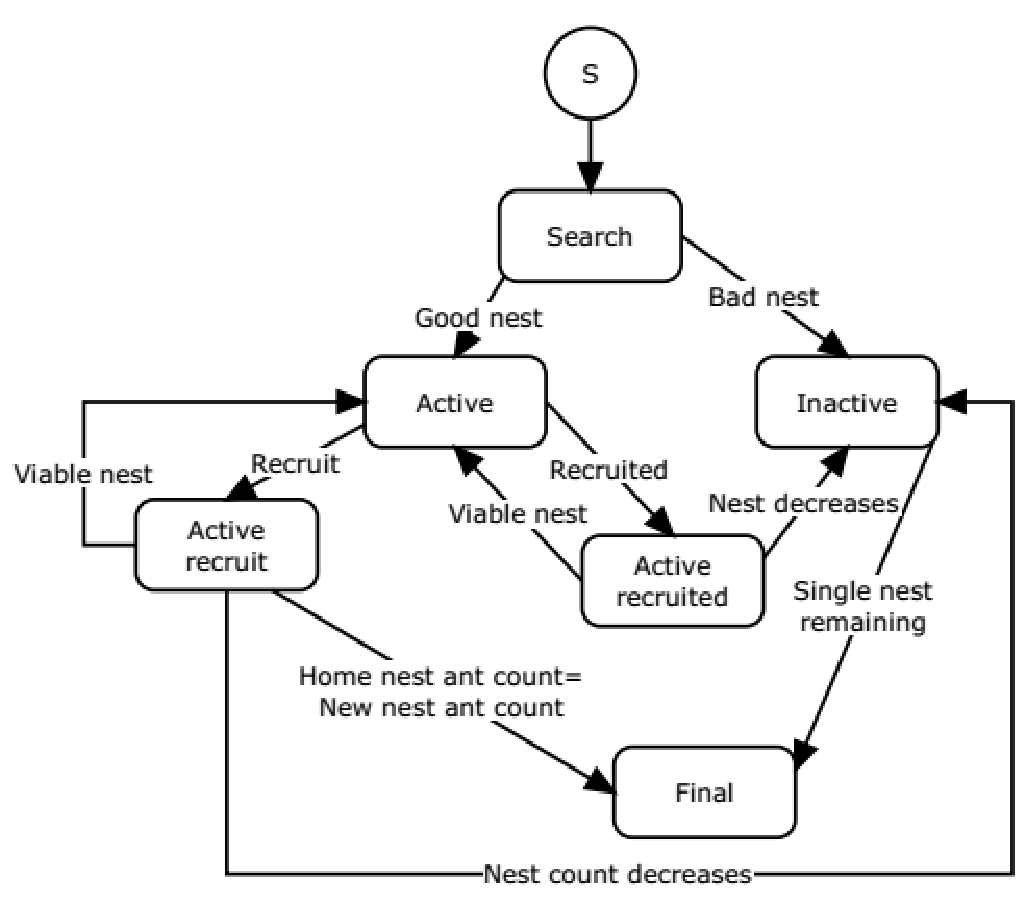
\includegraphics[width=0.9\linewidth]{aco_state}
	\caption{Ant House Hunting State Diagram}
	\label{fig:anthousehuntingstate}
\end{figure}

In the first round all house hunting ants initialize a nest and go to it. The ants then simulate the performance of the solution as described previously. If the simulated result's performance is under a given threshold, then the ant goes into the passive state, otherwise it goes into the active state.

In the second round, all ants return to the home nest and active ants try to recruit other ants at the home nest. Passive ants can not be recruited until the final round when all ants go to the single remaining nest. Active ants recruit randomly from the other active ants at the home nest by choosing another ant to recruit and bring it to it's committed nest. In order to ensure no conflicts between recruiting ants, the ants recruit iteratively and an ant which was already recruited does not recruit someone else. This recruitment is biased by the perceived suitability of the nest by the ants, such that better nests are given priority. The bias is achieved by sorting the ants by the perceived viability and then randomly choosing a recruiter ant such that ants with better suitability have a higher chance of being recruiters and ants with lower viability have a higher chance of being recruited. This is achieved using the following formula, where the probability of an ant to recruit is defined as the viability of the ant's chosen nest divided by the sum of all the ant's chosen nests.

\begin{equation}
p_{recruit} = ant_{viability} / \sum\limits_{i=1}^n ant_{viability}
\end{equation}

Once an ants recruits another ant the two ants go together to the nest of the recruiting ant. When reaching a new nest, active ants count the number of ants at the nest and check if the nest they reached is the same as the previous nest they went to. Based on the number of ants and the nest there are three cases:

\begin{enumerate}
	\item If the nest is the same nest that the ant went to before and the number of ants has increased or remained the same then the nest is still a possible solution so the ant updates the count and waits an extra round at the nest. After waiting a round, the ant checks if the number of ants at the home nest is the same as that at its current nest. If they are the same then the ant goes to the final state, new servers are added or removed and all ants morph back to ACO ants.
	\item If the nest is the same nest that the ant went to before and the number of ants has decreased then the ant becomes passive because the nest is in the process of being dropped out. The ant returns home in the same round that active ants wait at the new nest.
	\item If the nest is different then the nest the ant was committed to then the ant waits a round and then it checks to see if the number of ants at its new nest has decreased or not. If the number has decreased, then this nest is dropping out as the ants already committed to it have gone to the home nest and the ant becomes passive. Otherwise, the ant commits to its new nest and goes home to recruit other ants.
\end{enumerate}

The above algorithm can be described as follows in pseudo-code in Figure \ref{ant:pseudocodeHouseHunting}. $R_{x}$ represents round x.

\begin{algorithm}
\begin{algorithmic}
	\State $R_{1}$: Go to new nest
	\State Compute suitability of new nest
	\If{Suitability $<$ threshold}
		Switch to passive
	\EndIf
	\State $R_{2}$: Go to home nest
	\If{Ant is active \&\& Ant is not recruited}
		\State Recruit another ant
		\State Go to new nest
	\ElsIf{Ant is recruited}
		\State Go to new nest
	\EndIf
	\State $R_{3}$: Count number of ants at new nest = $count_{new}$
	\If{Nest is same and $count_{new} >= count_{old}$}
		\State Wait round
	\ElsIf{Nest is same and $count_{new} < count_{old}$}
		\State Switch to passive
		\State Go to home nest
	\ElsIf{Nest is different}
		\State Wait round
	\EndIf
	\State $R_{4}$: Count number of ants at new nest $count_{new}$
	\If{$count_{new} == count_{home}$}
		\State Switch to final state
	\ElsIf{$count_{new} < count_{old}$}
		\State Switch to passive
		\State Go to $R_{2}$
	\EndIf
	\State Return final state
	\State Switch ants to ACO ants
\end{algorithmic}
\caption{Ant House Hunting Pseudocode}\label{ant:pseudocodeHouseHunting}
\end{algorithm}

\subsection{Mathematical model: nest viability}

In order to determine if a nest should be considered as a solution ants must determine the viability of the nest. Because it is impossible for ants to predict how the user requests would be processed by more/less servers the ants use a heuristic to approximate the viability of each solution. It is important to note that due to each ant having a different memory of servers it has recently visited, different ants will see the same nest as having a different viability score.

There are two cases to consider - one when a cloud is over-loaded and servers should be added, and one where the cloud is under-loaded and servers should be removed.

\subsubsection{Over-loaded cloud}

In the case of an over-loaded cloud, each of the nests will have its solution contain more servers than the count of servers known by each ant. As such in order to determine the viability of the nest, the ant needs to simulate how a cloud with the extra servers would behave. The ant only has a short memory of its last $x$ visited servers and the amount of pheromone at these servers when it visited them. Because of this, the ant assumes that it would have visited the new servers with equal probability, so it replaces $y$ servers in its history with servers with optimal pheromone level, where the optimal pheromone level is defined as:

\begin{equation}
	p_{opt} = \frac{Pt_{max} + Pt_{min}}{2}
\end{equation}

and 

\begin{equation}
	y = x * \frac{newServerCount - cloudSize}{newServerCount}
\end{equation}

As such, the ant computes the average pheromone level across the last $x$ servers it would have visited as:

\begin{equation}
	p_{averageScaled} = \frac{y * p_{opt} + \sum\limits_{i=y+1}^x p_{i}}{x}
\end{equation}

Finally, the viability of the nest is defined as:

\begin{equation}
	viability = 1 - \frac{\left|p_{averageScaled} - p_{opt}\right|}{p_{opt}}
\end{equation}

With this approach, the ant simulates how the system would behave if it had $y$ extra servers taking some of the load from the existing servers. It then computes the viability based on how close the simulated pheromone is to the optimal pheromone.

\subsubsection{Under-loaded cloud}

In the case of an under-loaded cloud, each of the nests will have its solution contain less servers than the count of servers known by each ant. As such in order to determine the viability of the nest, the ant needs to simulate how a cloud with the lower count of servers would behave. The ant computes a number of servers $y$ in its history which should be removed as:

\begin{equation}
	y = x * \frac{cloudSize - newServerCount}{cloudSize}
\end{equation}

and then simulates the average pheromone for the cloud as:

\begin{equation}
	p_{averageScaled} = \frac{\sum\limits_{i=y+1}^x p_{i}}{x}
\end{equation}

The viability of the nest is calculated as in the case of the overloaded cloud. With this approach, the ant simulates how the system would behave if it had $y$ less servers and the remaining servers are taking the load from the removed servers. The viability is computed based on how close the simulated pheromone is to the optimal pheromone.

\section{Self-organizing algorithm conclusions}

The proposed approach for the self-optimizing control of cloud resources makes use of two self-organizing algorithms. The first algorithm is used in order to detect breaches of SLA before they happen such that proactive measures can be taken. The second self-organizing algorithm finds the optimal count of servers which should be running in the cloud.

The thesis uses the ACO algorithm to detect possible breaches of SLA by having ants continuously move through the network and measure the load on the network of servers. This is a novel approach as previous research has only focused on using the ACO to optimize various problems and not for detection of possible problems. The proposed approach ensures that the detection of SLA breaches can be done ahead of the actual breach while at the same time being fully scalable as the self-organizing algorithm scales with the number of servers.

The second algorithm which optimizes the number of servers in the cloud makes use of a different self-organizing approach also inspired by the behaviour of ants. This algorithm is also novel as previous research into the house hunting algorithm was only used as a way to model the behaviour of ants and not for problem optimization.

The following chapter will introduce the test bed and simulation environment used to test the algorithms and also present results for the implementation of the self-optimizing self-organizing cloud.
